\documentclass{IEEEtran}
\usepackage[utf8]{inputenc}
\title{Resultados Tarea 4 Métodos Computacionales }
\author{Diego Felipe  Martinez Valencia}
\date{\today}
\usepackage{natbib}
\usepackage{parskip}
\usepackage{fancyhdr}
\usepackage{float}
\usepackage{graphicx}
\usepackage{subfigure}
\providecommand{\abs}[1]{\lvert#1\rvert}
\providecommand{\norm}[1]{\lVert#1\rVert}
\setlength{\textwidth}{170mm}
\setlength{\textheight}{230mm}
\setlength{\topmargin}{-20mm}
\setlength{\oddsidemargin}{-1mm}
\setlength{\evensidemargin}{30mm}
\usepackage{ragged2e}
\usepackage[usenames, dvipsnames]{color}
\usepackage[english]{babel}
\usepackage{color}
\begin{document}
\maketitle{}
\vspace*{-1cm}
\justify 
\section*{ODE}
En esta sección de muestran las gráficas de resultados del ejercicio de ecuaciones diferenciales ordinarias.
\begin{equation}
    \frac{d^{2}\vec{v}(t)}{dt^{2}}=-\vec{g}-c\frac{|\vec{v}(t)|^{2}}{m}\frac{\vec{v}(t)}{|\vec{v}(t)|}
\end{equation}
Inicialmente, para este caso se asignaron las siguientes condiciones iniciales:
\begin{equation}
    \vec{x}(t=0)=(0,0) \quad \vec{v}(t=0)=300(cos(\phi),sin(\phi))
\end{equation}
\subsection{Gráfica con ángulo de 45$^\circ$}
\begin{figure}[h]
    \centering
    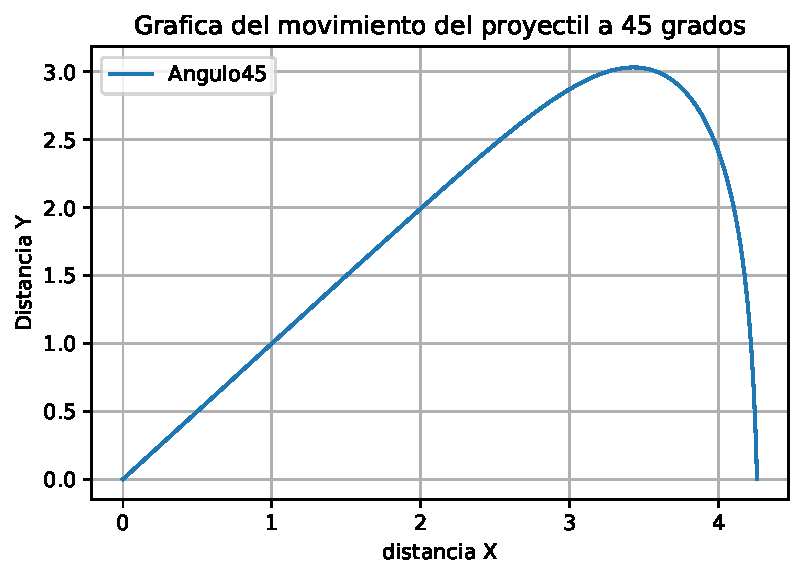
\includegraphics[scale = 0.6]{ODE_45grados.pdf}
    \caption{Gráfica de movimiento a 45 grados}
    \label{fig:my_label}
\end{figure}
De esta gráfica de la figura 1 es posible verificar que la distancia alcanzada es aproximadamente 7.95m. EN esta gráfica es posible ver un movimiento parabólico que sigue la partícula en movimiento, no está demás aclarar que este movimiento(como se vé en fisica 1) está dado por las fuerzas que actúan sobre la partícula. Aunque no se trate de meramente un problema de física 1, sino que el movimiento sea descrito como una ecuación diferencial ordinaria, la física detrás de este fenómeno es la misma y dado esto se debe tener una respuesta similar a como se haría en un ejercicio que ponga Juan Gabriel cuando dicta física 1. :) 
\subsection{Gráfica con ángulos variables$^\circ$}
Con las mismas condiciones iniciales de la anterior figura:
\begin{equation}
    \vec{x}(t=0)=(0,0) \quad \vec{v}(t=0)=300(cos(\phi),sin(\phi))
\end{equation}
\begin{figure}[h]
    \centering
    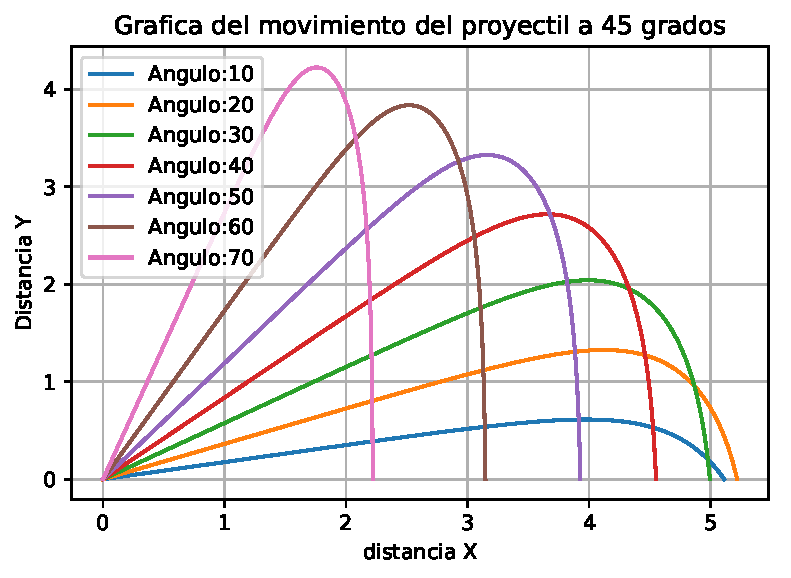
\includegraphics[scale = 0.6]{ODE_varicion_grados.pdf}
    \caption{Gráfica de movimiento a diferentes ángulos}
    \label{fig:my_label}
\end{figure}
De esta gráfica de la figura 2 es posible verificar que la distancia máxima alcanza se da cuando se tiene un ángulo de 20 grados.

\section*{PDE}
Comportamiento de la temperatura en una sección de una roca de calcita con una varilla cilíndrica incrustada perpendicularmente de diámetro 10cm. La ecuación que representa el sistema es la siguiente:

\begin{equation}
    \frac{dT(x,y)}{dt}=\nu\frac{d^{2}T(x,y)}{dx^{2}}+\nu\frac{d^{2}T(x,y)}{dy^{2}}
\end{equation}

La varilla posee una temperatura de 100$^{\circ}C$ constantes. Las condiciones iniciales de temperatura para la roca de calcita es de 10$^{\circ}C$ y las condiciones de frontera se dan para diferentes casos. Para cada caso, se realizo una simulación para un T = 1000*dt, con un dt = $ alpha*pow(dx,2)/v;$ donde v = $k_d/(Cp*rho)$. En cada uno, se realzaron 4 cuatro gráficas, que constatan la evolución de la temperatura en diferentes puntos del tiempo.

\end{document}